\documentclass{vgtc}                          % final 

%% to provide the the path and extension of a graphics file:
%% \includegraphics{diamondrule} is completely sufficient.
%%
\ifpdf%                                % if we use pdflatex
  \pdfoutput=1\relax                   % create PDFs from pdfLaTeX
  \pdfcompresslevel=9                  % PDF Compression
  \pdfoptionpdfminorversion=7          % create PDF 1.7
  \ExecuteOptions{pdftex}
  \usepackage{graphicx}                % allow us to embed graphics files
  \DeclareGraphicsExtensions{.pdf,.png,.jpg,.jpeg} % for pdflatex we expect .pdf, .png, or .jpg files
\else%                                 % else we use pure latex
  \ExecuteOptions{dvips}
  \usepackage{graphicx}                % allow us to embed graphics files
  \DeclareGraphicsExtensions{.eps}     % for pure latex we expect eps files
\fi%

%% it is recomended to use ``\autoref{sec:bla}'' instead of ``Fig.~\ref{sec:bla}''
\graphicspath{{figures/}{pictures/}{images/}{./}} % where to search for the images
\usepackage{accents}
\usepackage{microtype}                 % use micro-typography (slightly more compact, better to read)
\PassOptionsToPackage{warn}{textcomp}  % to address font issues with \textrightarrow
\usepackage{textcomp}                  % use better special symbols
\usepackage{mathptmx}                  % use matching math font
\usepackage{times}                     % we use Times as the main font
\renewcommand*\ttdefault{txtt}         % a nicer typewriter font
\usepackage{cite}                      % needed to automatically sort the references
\usepackage{tabu}                      % only used for the table example
\usepackage{booktabs}                  % only used for the table example
\usepackage{url}
\usepackage{float}
%% OnlineID. Otherwise, you may safely leave it at ``0''.
\onlineid{0}

%% declare the category of your paper, only shown in review mode
\vgtccategory{Research}

%% allow for this line if you want the electronic option to work properly
\vgtcinsertpkg

%% In preprint mode you may define your own headline.
%\preprinttext{To appear in an IEEE VGTC sponsored conference.}

%% Paper title.

\title{M4: Final Submission}

%% This is how authors are specified in the conference style

%% Author and Affiliation (single author).
%%\author{Roy G. Biv\thanks{e-mail: roy.g.biv@aol.com}}
%%\affiliation{\scriptsize Allied Widgets Research}

%% Author and Affiliation (multiple authors with single affiliations).
%%\author{Roy G. Biv\thanks{e-mail: roy.g.biv@aol.com} %
%%\and Ed Grimley\thanks{e-mail:ed.grimley@aol.com} %
%%\and Martha Stewart\thanks{e-mail:martha.stewart@marthastewart.com}}
%%\affiliation{\scriptsize Martha Stewart Enterprises \\ Microsoft Research}

%% Author and Affiliation (multiple authors with multiple affiliations)
\author{Nicole Cherches\\
\scriptsize Matr. Nr.: 01506832
\and Alexander Gelb\\
\scriptsize Matr. Nr.: 01268620
\and Benjamin Neckam\\
\scriptsize Matr. Nr.: 01301917
\and Axinya Tokareva\\
\scriptsize Matr. Nr.: 01368965
}

%% A teaser figure can be included as follows, but is not recommended since
%% the space is now taken up by a full width abstract.
%\teaser{
%  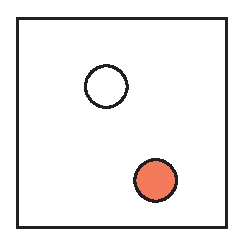
\includegraphics[width=1.5in]{sample.eps}
%  \caption{Lookit! Lookit!}
%}

%% ACM Computing Classification System (CCS). 
%% See <http://www.acm.org/about/class> for details.
%% We recommend the 2012 system <http://www.acm.org/about/class/class/2012>
%% For the 2012 system use the ``\CCScatTwelve'' which command takes four arguments.
%% The 1998 system <http://www.acm.org/about/class/class/2012> is still possible
%% For the 1998 system use the ``\CCScat'' which command takes four arguments.
%% In both cases the last two arguments (1998) or last three (2012) can be empty.

\CCScatlist{
  \CCScatTwelve{Visu\-al\-iza\-tion}{Visu\-al\-iza\-tion techniques}{}{};
  \CCScatTwelve{GAIA}{ESA}{}{}
}

%%%%%%%%%%%%%%%%%%%%%%%%%%%%%%%%%%%%%%%%%%%%%%%%%%%%%%%%%%%%%%%%
%%%%%%%%%%%%%%%%%%%%%% START OF THE PAPER %%%%%%%%%%%%%%%%%%%%%%
%%%%%%%%%%%%%%%%%%%%%%%%%%%%%%%%%%%%%%%%%%%%%%%%%%%%%%%%%%%%%%%%%

\begin{document}

%% The ``\maketitle'' command must be the first command after the
%% ``\begin{document}'' command. It prepares and prints the title block.

%% the only exception to this rule is the \firstsection command
\firstsection{Motivation}
\maketitle
On 19th December 2013 the "European Space Agency", ESA, launched  the "Gaia"-satellite to gather more information about our galaxy and create a three dimensional map out of it. Since then data like velocities, positions, errors, parallax and many more were collected of about 2 million stars. All together each star has more than 50 features in the data set which means the amount of entries is extremely high.\\
But working with such a huge data set is not easy and most of the time not necessary because scientists only want to focus on a specific area of the galaxy. Therefore they only use subsets of the data. Now the idea was, to take the whole data set and don't look into detail but see the "big picture" and try to find patterns, correlations, outliers or other interesting things.\\
This could be useful for scientists who are not sure which part of the data they want to explore and for example can focus only on the anomalies or other fascinating sections in the data set.

\section{Related Work}
What we first did, was searching for similar problems and finding out, what other visualizations looked like in this area. Most of the space visualizations we found online, were 3d simulations of the galaxy. Examples of them are the ESA Star Mapper\cite{starmapper} or 100000 stars\cite{chromeexperiment}. They both are 3d interactive simulations of the stellar neighbourhood.
We also found a 2d-visualization from the ESA, which visualizes the stars from the Gaia data set\cite{gavs}, also in 3d.
But we couldn't find anything that has to do with correlations or patterns. All the existing visualizations are showing the stars themselves with their exact location.
So we started prototyping and in the end we even used some of our first basic ideas in our final system.
After that, we focused on finding existing visualization systems. In the VIS course we already learned about Tableau\cite{tableau}, which allows the user to import Data and create visualization plots based on it. And we also found out about a software named Glue\cite{glue}, which helps to create plots and analyze relationships between different data.
So we basically tried to create a mixture of both tools and started designing our own system.

\begin{figure}[h]
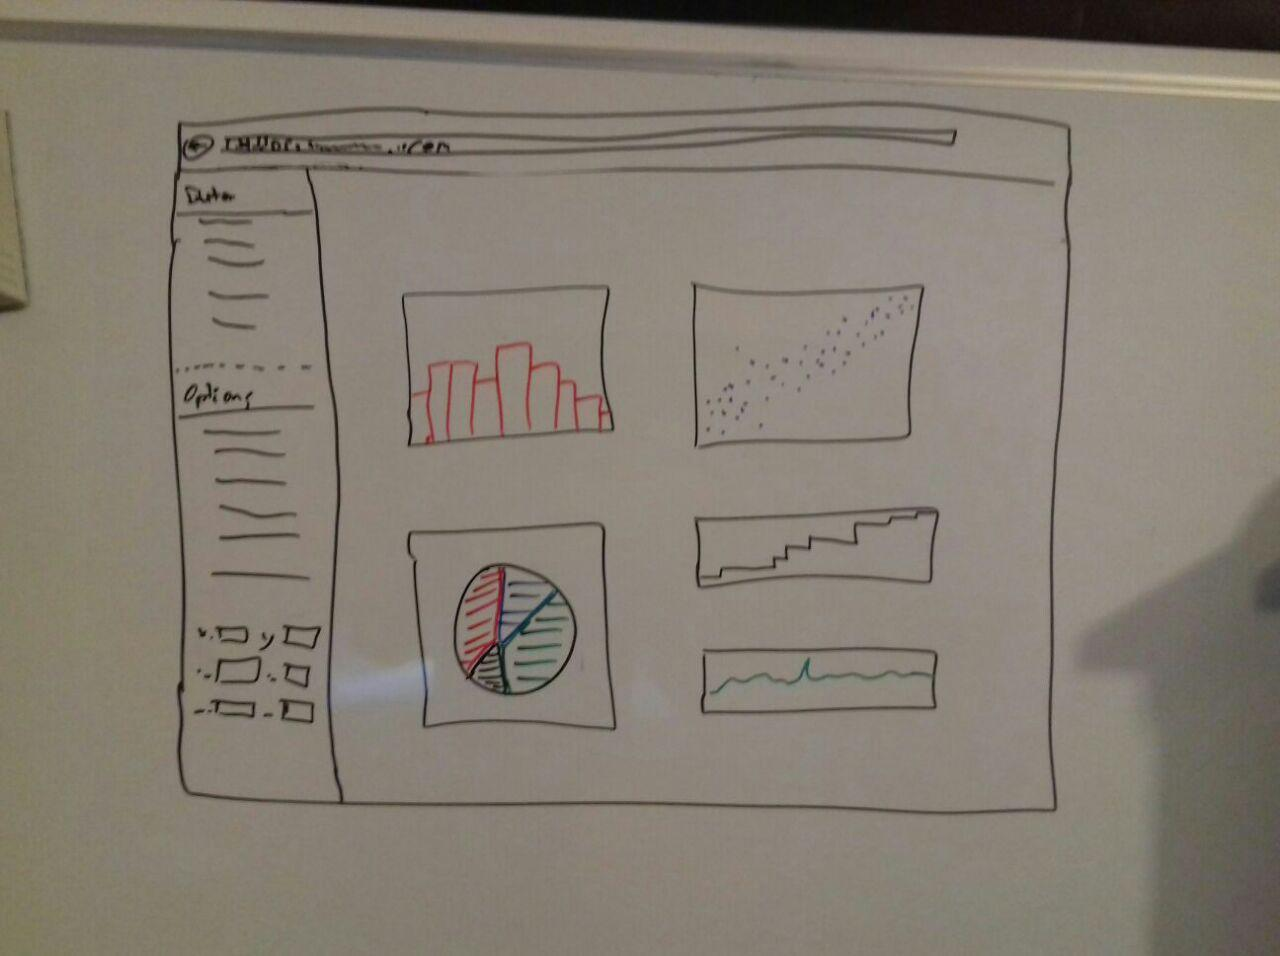
\includegraphics[width=0.5\textwidth]{Prototype1.jpg}
\centering
\caption{Lo-Fi Prototype of our user interface}
\end{figure}

Figure 1 is a picture, that shows how we imagined the visualization system at the beginning.
As we will see later in the end product, our Lo-Fi Prototype looks similar to our visualization system. We kept the sidebar, where the user has basic information about the data and can choose options on how the data will be presented. Also the diagrams and plots appear all on one screen so the user can see how they correlate. What we didn't do, is creating different plots next to each other. We mixed different plots together into one, so it is easier to see the patterns. Also our first idea was also creating one plot in 3d, but realized later, that we don't need it for our system. However, instead of focusing on the meaning of the data, we focused on exploring the data itself, because we didn't know anything about it.

\section{Approach}
When we first thought about our visualization design, we tried to think about our user. The system should help to analyze "the big picture" of the Gaia data set and not only details. So, we thought about plots that could help us to accomplish that.

Anyway, the best idea was to implement a scatterplot matrix: It fits into our project well, because we can see a whole grid filled with Scatterplots, showing all correlations between selected data values.
The user has to choose a set of columns from the data set. The scatterplot matrix contains histograms in the diagonal, so the user can find patterns even better.

\section{Implementation}
The whole program was written in JavaScript combined with CSS and mainly designed for Google Chrome. For the front-end we decided to use the toolkit "Bootstrap"\cite{bootstrap} which provides different templates so we didn't have to spend too much time for designing the user-interface.\\
To visualize the data the JavaScript library "D3"\cite{d3} was used which offers the ability to let the developer interact with the data.\\
\\
We encountered many problems which challenged us to implement things properly. One of the problems were filtering the data, so that we don't have any undefined values, which would cause problems and errors. We figured out that we cannot just delete all the entries, which contain a NULL or any other non valid value, because this would reduce the data set to almost zero entries. Therefore, we went through the documentation of the data set and tried to figure out which features of the stars can be excluded and which not. Unfortunately we could not filter out all unnecessary values at the beginning , we had to do a "pre-filtering" to remove all non-integer values and afterwards almost every function had to do their own filtering to adapt the data to their specific task.\\
To minimize the data set, we got the hint to have a look on "principal component analysis" which can help to reduce the dimensions. At the beginning we had the idea to implement a plugin\cite{pca} for D3 which processes the input data first and then work with it. But after implementing successfully we recognized that the produced result was not what we had in mind. It was built for data sets with less dimension than we have and therefore the performance was tremendously slow. So we focused on "DimStiller"\cite{dimstiller} and tried to work with it. Basically it almost fulfilled our requirements but unfortunately it doesn't offer an API to connect it to our application. Due to time issues, we weren't able to create a pipeline, where the input file is send to DimStiller, which processes it and then sent back to our application, where the user can work with a trimmed file. Although it is not realised yet, we were curios how the result of DimStiller would look like and played around with it a little bit and decided to present the outcome here.\\
DimStiller's principal component analysis consists of five so called steps, which happen consecutively. These are "Cull:Variance", "Data:Normalize", "Collect:Pearson", "Reduce:PCA" and "View:SPLOM". The first interesting and a little bit disappointing result appeared at "Collect:Pearson", which shows the correlation between the dimensions. It reduced the dimension from 52 to 28 dimension. When we look on figure 2, we see that most of the dimensions do not correlate, although we expected more correlation, since the amount of data is enormous.\\
At the "Reduce:PCA" step, one can choose interactively the final number of dimensions via the user interface, which is shown in figure 3. The problem here is, that most dimensions are combined and we are not sure, how much and if there is an information loss. Due to this fusion the old names of the columns are discarded and get new names like "S4.D1", like we in figure 4 on the x-axis. Furthermore we can see that the picture concerning the correlations didn't change, there are no or just slight correlations among the new dimensions.
\begin{figure}[H]
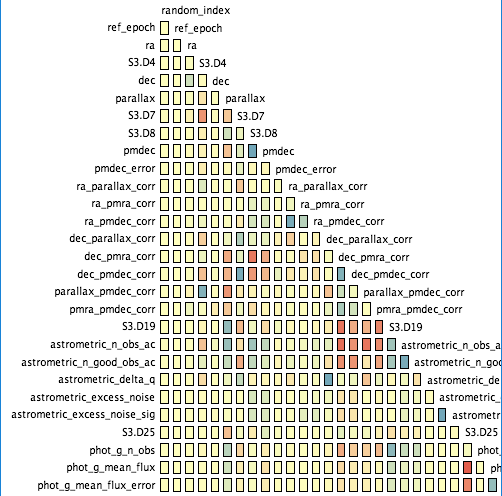
\includegraphics[width=0.5\textwidth]{pearsoncoeff.PNG}
\centering
\caption{Pearson coefficient, where blue means positive correlation, yellow no correlation and red negative correlation}
\end{figure}
\begin{figure}[H]
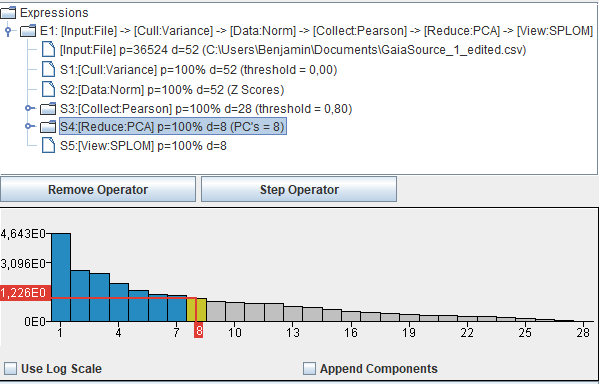
\includegraphics[width=0.5\textwidth]{pca.PNG}
\centering
\caption{PCA step}
\end{figure}
\begin{figure}[H]
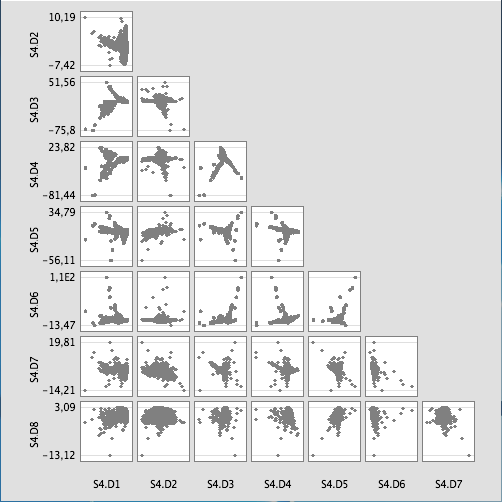
\includegraphics[width=0.5\textwidth]{splom.PNG}
\centering
\caption{Scatterplot matrix with reduced dimension to 8}
\end{figure}


As correlations are a major part in this project, we needed a way to compute correlations between columns in our big data set.
So we used the formula for the correlation coefficient.\cite{corr}
\\
\\
$\rho_x{}_y$ = $\frac{\sum_{i=1}^n ((x_i-\overline{x}_n)(y_i - \overline{y}_n)}{\sqrt{\sum_{i=1}^n (x_i - \overline{x}_n)^2\sum_{i=1}^n(y_i - \overline{y}_n)^2}}$
\\
\\
This function is used for the scatterplot matrix.
The hard part about this, was that the formula is long and nested, so it was hard to compute it in D3. Also it was difficult to debug this function because of the size of the data set. Another challenge, was the right filtering of our data. For computing the correlation, we had to filter out empty entries or NaN values without modifying the data set too much.

\section{Results}
The first thing the user will probably look on, is the information about the Gaia data set. The name, number of rows and columns is displayed on the top left in the sidebar. \\

\begin{figure}[H]
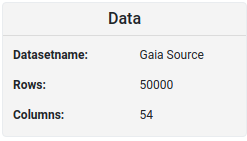
\includegraphics[width=0.3\textwidth]{1d.png}
\centering
\caption{data set overview}
\end{figure}

 This sidebar contains also the Options: Here the user can choose the Columns, he wants to analyse. He can select from all the columns in the Gaia data set. In this scenario our user wants to see the correlations between the columns "ra", "dec", "astrometric\_n\_obs\_al" and "l".
 
\begin{figure}[H]
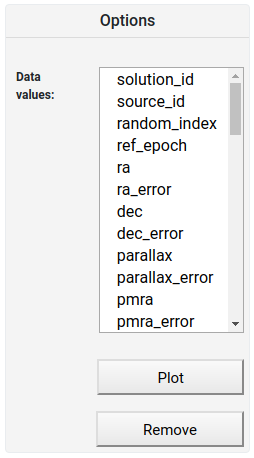
\includegraphics[width=0.2\textwidth]{options.png}
\centering
\caption{Options}
\end{figure} 
 
Then he presses "plot" and the Scatterplot Matrix is displayed on the site.

\begin{figure}[H]
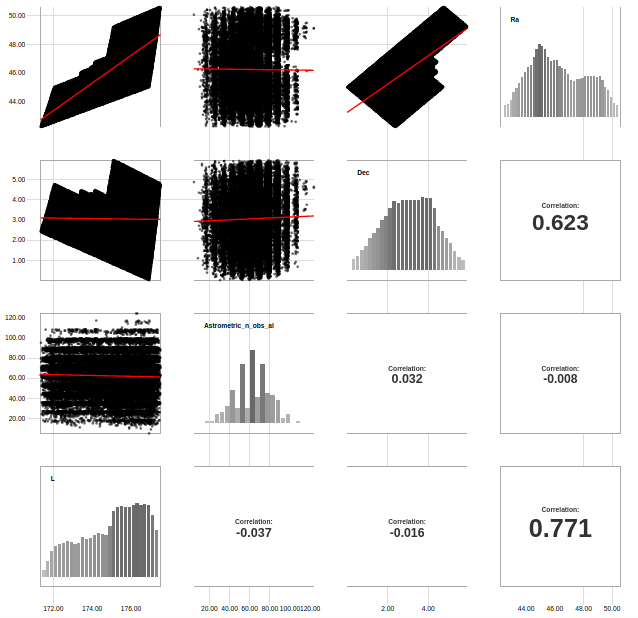
\includegraphics[width=0.5\textwidth]{scattermatrix.png}
\centering
\caption{Scatterplotmatrix}
\end{figure}

\begin{figure}[H]
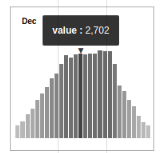
\includegraphics[width=0.3\textwidth]{tooltip.png}
\centering
\caption{Cell with Tooltip function}
\end{figure}

As said before, now he can see all the columns at a glance in one big view. The correlations between all the columns are computed and displayed as Scatterplots with regression lines in the upper half of the Matrix, the values in the lower half. In the diagonal he can see histograms showing the distribution in the columns, also they have the column names in the title. When hovering over the bars, he can read the exact value of the bar. Hovering over the correlation value, displays the two column names, which where analysed. To clear the view, he can press "remove" and select new columns to plot. Or he just plots a new matrix underneath the old one.
\section{Discussion}
The main strength of our visualization project is, that the user has a fast overview, where he can see all the patterns and has "the big picture" of the data set. With the Scatterplot Matrix, he already can see how a set of columns correlates with each other, but that's not it: There are also histograms in the diagonal of the Matrix, which help understanding the data better. Also we implemented a regression line for the scatter plots. We are using tooltip for displaying further information about plot objects and a filter, so the user can manually choose what he wants to see and ignore the rest. The visual strengths of our project are the simple design, because we only use few colours ("Less is more!"). 
The weakness of the design is the weak performance. The size of the data set is a big problem, so it takes a lot of time to display the plots with so many points with Javascript and D3. Also we had a time management problem and couldn't achieve all that we wanted to do in this project (e.g. the PCA). 
\subsection{Lessons learned}
\subsubsection{Nicole Cherches}
There were a lot of things, I learned from the Gaia project. First of all, I would like to talk about the technical aspects: As this was my first visualization task, it was a whole new experience for me to work with d3 and Javascript. But the most important part is, that I learned how to work with a huge data set and how to get the most out of it. We first tried to learn everything about it, also we realized that Astronomy is too complicated for us to understand. After our talk with Mr. Moeller, we then tried another approach: We did a data exploration task, which is all about getting to know a huge data set, we don't know much about.  
Another important part, I learned from this project, was working in a group. I learned a lot about coordination, planning and distributing tasks. This is also a good lesson, because collaboration with others is a necessary skill in computer science.
\subsubsection{Alexander Gelb}
For me the most interesting part of this project was, to learn how to visualize a big data set with the d3 library. It was very interesting to work with such a huge set with different information about the stars in our galaxy, altough we are not familiar with the values inside the gaia data. I was very excited about working with Joao Alves and Irati Larreina, who are both operating in the domain of astronomy. I learned a lot from Irati about this domain and together with my project team and Irati we produced a nice little app which shows hopefully useful information for her future work. \\
The most difficult part for me was to fix the performance problem. For this I still was not able to solve this problem, but maybe D3 is not the best option to handle such a big amount of data.
\subsubsection{Benjamin Neckam}
There were two things I will take out of this project.\\
The first one refers to the implementation and the chosen programming language. Basically I was not very used to JavaScript, to be more precise, I had no experience with it, but I was really impressed by "D3". The opportunities you have to visualize data are brilliant and allow the programmer to choose over a wide variety of plot types. The only disadvantage that really falls into weight was the performance. If the data set is bigger than, let's say, 100.000 entries it takes some time to calculate and plot the data and in our case the file contains more than ten times more entries. But all in all it was very interesting and in my opinion very important for my future to work with JavaScript and "D3" and get deeper into this part of front end programming.\\
The second part is about the collaboration between the project group of the class and research group of another university. Until now all the projects at the university were from the teachers of the faculty itself but in this case the task was from the "Universitätssternwarte Wien". This means, we had to arrange meetings with the project leader and a student which also is a member of the research group and talk about the task in detail and what the aim of this project is. It was fun and interesting to meet all these people but I recognized that, even if there are not too many people involved it can easily happen, that confusion arises. Like in our case, we started to focus on the wrong details and parts and had to "restart" our project. Therefore, I would say communication is the most important part in a project, especially if it is a collaboration of two or more groups, I guess this is the biggest lesson I learned from the project.
\subsubsection{Axinya Tokareva}
I would like to take out a few positive points. First of all, it was a good experience with JavaScript in general, and with the D3-library. Surprisingly, the D3 was quite convenient and easy to understand for data processing and visualization, but its performance is not a good side.\\
Secondly, I worked with such a huge data set for the first time. It was interesting to understand how to work with it and what to focus on.\\
Third, I think working in a group is one of the important lessons I learned. I comprehended how important it is to plan your time and distribute the work to the group members in time.
\section{Separation of Tasks}
Nicole Cherches: Report, Corrrelation analysis\\
Alexander Gelb: Scatterplots, Regression line\\
Benjamin Neckam: Report, Principal Component Analysis\\
Axinya Tokareva: Histograms, insert correlations in scattermatrix, Tooltips, Scales
\bibliographystyle{unsrt}
\bibliography{reference}

\end{document}